\chapter{Study and Results}
In this chapter we will present the study that has been performed and the results
generated using our simulation.

\section{ADHD and Personality Traits}
A recent study \cite{Polanczyk2015} shows that the world wide prevalence
for anxiety disorders within children and adolescents to be around 6.5\%, and 
Attention-deficit hyperactivity disorder \textbf{(ADHD)}\cite{Barkley1997} being one
of the most common childhood behavioral disorder, ranging between 5-10\% \cite{Sayal2018}.

\bb

Because of the high prevalence of anxiety disorders in the general population,
and the availability of studies correlating ADHD with personality traits, we
decided to study the effect of children with personality profiles that match those
of ADHD patients on the class as a whole.

\bb

The primary reference for how ADHD symptoms relate to personality traits, we took
from \cite{Nigg2002}, where the authors write

\textit{\dots our findings for the two major symptom domains suggest the following
conclusion: overall ADHD symptoms are related to low Conscientiousness, low Agreeableness, and high Neuroticism.}

\section{Study Description}
The study we performed had the objective to simulate how an increasing number of
students with ADHD symptoms would affect the group dynamics. This was achieved by
the following steps.

\begin{itemize}
    \item We defined three types of students (\textit{ADHD, Normal, Ambitious})
    \item Created several classroom profiles varying the ratio of the different student types present
    \item Run a Simulation study comparing the classroom profiles to each other
\end{itemize}

\subsection{Student Types}
The student types chosen have been inspired by the literature, whereby we 
took defined a ADHD student using results from \cite{Nigg2002}, a normal type using
\cite{Srivastava2003} and Ambitious students from \cite{Asendorpf2003}.

At this point it is worth to note that the defined student types are prototypical in nature.
There exists no \textit{normal} nor \textit{ADHD} personality trait type. The Big-Five
model is a continuos scale in all five dimensions. The different personality types
have been defined as a shorthand to simplify the analysis of results and highlight
the divergence between groups.

The concrete personality profiles used for each type are found in table \ref{StudenTypesTable}

\begin{table}[h!]
    \centering
    \begin{tabular}{|l|c|c|c|c|c|} 
        \hline
        \textbf{Student Type} & \textbf{O} & \textbf{C} & \textbf{E} & \textbf{A} & \textbf{N} \\
        \hline
        \hline
        ADHD & RND & 0.20 & RND & 0.20 & 0.80 \\
        \hline
        Normal & 0.75 & 0.60 & 0.55 & 0.65 & 0.50 \\
        \hline
        Ambitious & 0.80 & 0.80 & RND & 0.80 & 0.20 \\
        \hline
        Random & RND & RND & RND & RND & RND \\
        \hline
    \end{tabular}
    \caption{Table with Student types composition groups}
    \small RND indicates a random value from a uniform distribution between [0, 1]
    \label{StudenTypesTable}
\end{table}

\subsection{Groups}
Based on the student types we created various classrooms that where compared to
each other. Each group consisted of 30 students, varying the \% of each Student
type per group (see table \ref{GroupTable}).

The ratio of ADHD students is very high and does not correspond directly to
empirical findings (see \cite{Sayal2018} who estimates ratios to be between 5-10\%).
We have chosen those high values because ADHD is no black or white form of psychological
disorder, but rather a spectrum that can vary strongly in its intensity and persons behavior.
Similar to the student types, the different groups have been defined to exemplify
tendencies and highlight differences.

In addition the group 'Random' serves as a form of estimation how strong the simulation
output is affected by the classroom profile.

\begin{table}[h!]
    \centering
    \begin{tabular}{|l|c|c|c|c|} 
        \hline
        \textbf{Group} & \textbf{ADHD} & \textbf{Normal} & \textbf{Ambitious} &  \textbf{Random} \\
        \hline
        \hline
        ADHD-Low & 7\% & 93\% & 0\% & 0\% \\
        \hline
        ADHD-Medium & 17\% & 83\% & 0\% & 0\% \\
        \hline
        ADHD-High & 33\% & 66\% & 0\% & 0\% \\
        \hline
        ADHD-VeryHigh & 50\% & 50\% & 0\% & 0\% \\
        \hline
        ADHD-None & 0\% & 100\% & 0\% & 0\% \\
        \hline
        ADHD-None-Ambitious & 0\% & 50\% & 50\% & 0\% \\
        \hline
        ADHD-Low-Ambitious & 7\% & 46\% & 46\% & 0\% \\
        \hline
        ADHD-Medium-Ambitious & 20\% & 40\% & 40\% & 0\%\\
        \hline
        ADHD-VeryHigh-Ambitious & 50\% & 0\% & 50\% & 0\%\\
        \hline
        Random & 0\% & 0\% & 0\% & 100\% \\
        \hline
    \end{tabular}
    \caption{Groups composition studied}
    \small RND indicates a random value from a uniform distribution between [0, 1]
    \label{GroupTable}
\end{table}

\section{Results}
We have been simulating each of the groups defined above using 10 replicas, initiated
with different seed values.

The HA-Plot generated by the last step of the Data Analysis is shown in figure \ref{StudyResults}.

\begin{figure}[H]
    \makebox[\textwidth][l]{%
    \begin{minipage}[t]{500pt}
        \centering
        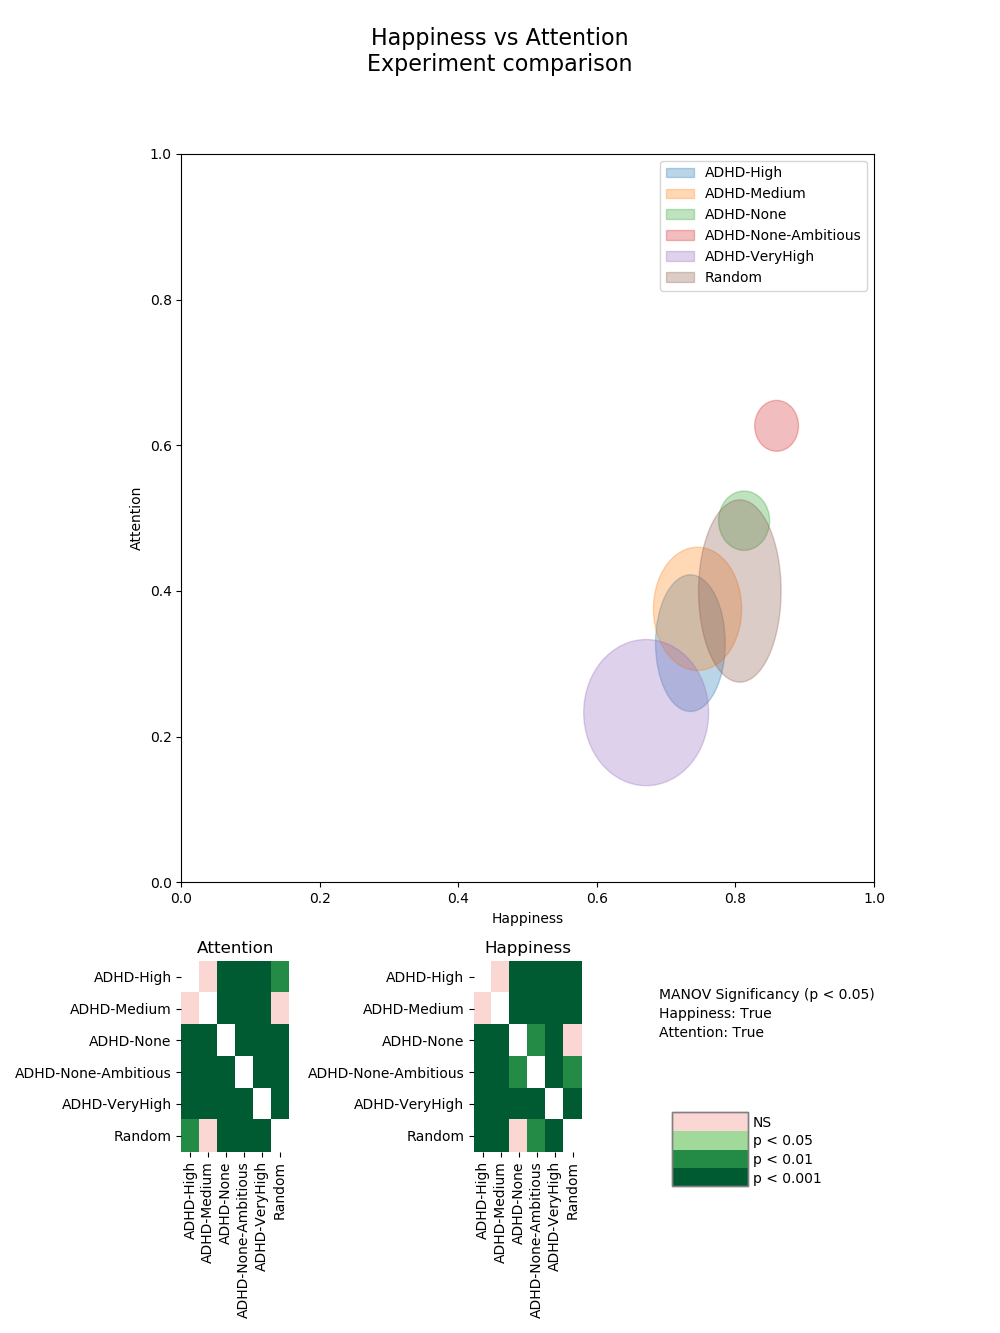
\includegraphics[width=400pt]{results/HAPlot}
    \end{minipage}    
    }%
    \caption{HA-Plot comparing the different classroom configurations}
    \label{StudyResults}
\end{figure}

Classrooms with ADHD students had a strong effect in all groups. The general
tendency seems to be that the higher the ratio of ADHD students, less happy and
attentive the class as a whole becomes. The ambitious students on the other
side cause the exact reverse effect, increasing happiness and attention.

\subsection{ADHD Effect}
Given this dynamic, specially the groups containing a mixture of ADHD and
ambitious students is interesting. Comparing the groups \textit{ADHD-Low-Ambitious},
\textit{ADHD-Medium-Ambitious} and \textit{ADHD-VeryHigh-Ambitious} shows that ADHD
type students have a far stronger effect than their ambitious counterparts.

\bb

This effect is most visible in the \textit{ADHD-Low-Ambitious} group, in which only
very few ADHD students, reduce mean happiness and attention compared to the \textit{ADHD-None}
group despite the presence of many more ambitious students.

\bb

\subsubsection{ADHD and Personality traits}
To investigate this further, we have calculated the correlation between student personality
traits and happiness, attention and conformity. The correlation matrix is part
of the HA-Plot of the final results (see figure \ref{StudyResults}). In addition we have calculated
two more correlation matrices, that contain all ADHD classrooms in one matrix, and
all None ADHD classes in the other (see figure \ref{CorrleationComparison}).

\bb

It appears that for None-ADHD Classrooms, the different personality traits are equally
correlated with the mean happiness and attention of the students. For the ADHD
classrooms on the other side there is a strong correlation for some of them, but not
for others. Happiness and Attention correlates strongly with Conscientiousness, Agreeableness
and Neuroticism; which by the way are the main personality traits for the ADHD student
type. This strong correlation between the key ADHD personality traits and the HA
axis explain the direction of the effect.

\bb

Concerning the strength of the effect, it is interesting to look at the HA-Plots
showing the individual agents of a single simulation Instance. Comparing the classroom
configurations \textit{ADHD-Low-Ambitious}, \textit{ADHD-Medium-Ambitious} and
\textit{ADHD-VeryHigh-Ambitious} contained in the Appendix (see figure \ref{results:LA-HAPlot}, \ref{results:MA-HAPlot} and \ref{results:VHA-HAPlot}),
one can see clearly that ADHD students and none-ADHD students are in separate clusters.
The ADHD agents in the lower left quadrant and the None-ADHD agents in the upper right quadrant of the plot.
As the ratio of ADHD students increases, the None-ADHD cluster is shifting
towards the lower left (less happy, less attention), while the ADHD cluster remains
where it was.

\bb

It appears that the ADHD students cause a strong shift in behavior of the None-ADHD
agents, without altering or adapting their own.

\begin{figure}[]
    \centering
    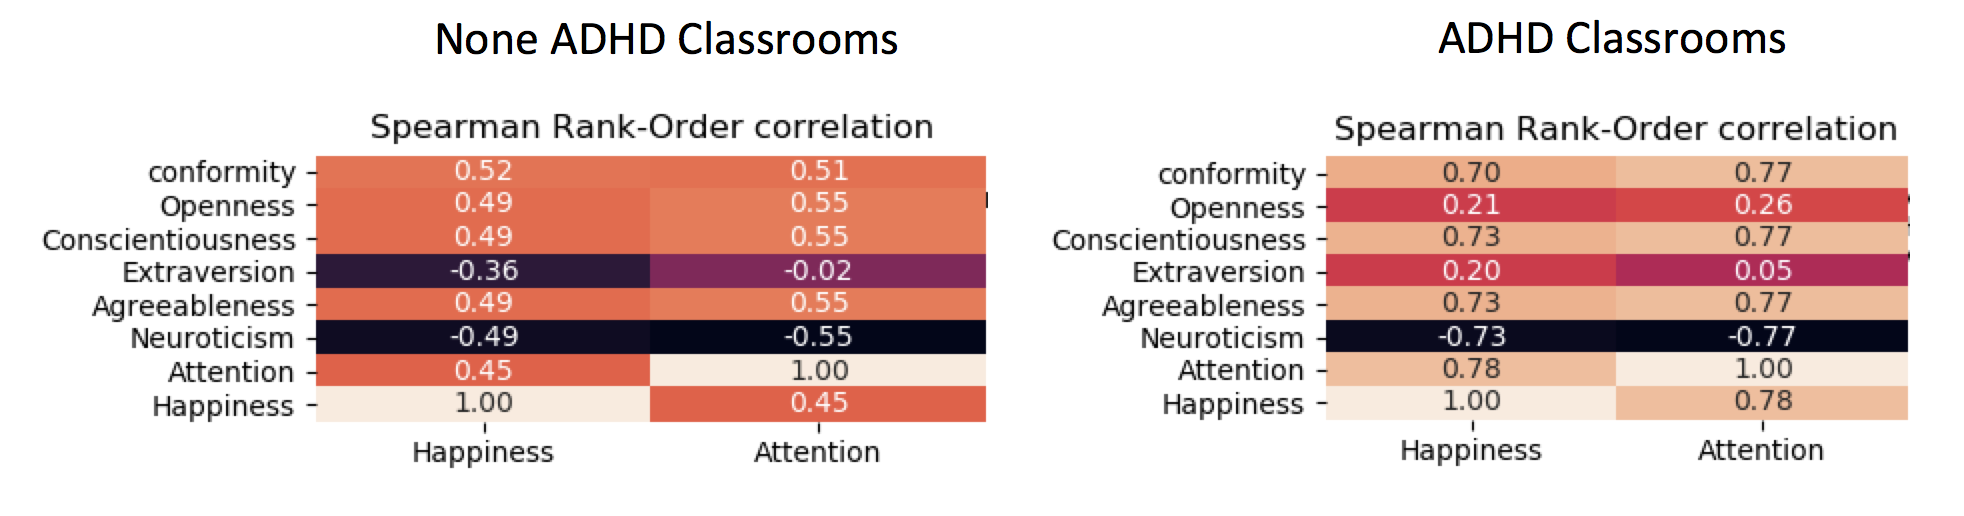
\includegraphics[width=400pt]{results/CorrelationComparison}
    \caption{Comparing change in correlation between ADHD and None-ADHD Classrooms}
    \label{CorrleationComparison}
\end{figure}

\subsection{Classroom riots}
Finally we want to shortly compare the classroom aggregate plots of the classroom
configurations \textit{ADHD-High} (see figure \ref{result:H-Classroom}), \textit{ADHD-None}(see figure \ref{result:N-Classroom}),
\textit{ADHD-None-Ambitious}(see figure \ref{result:NA-Classroom}) and \textit{ADHD-Low-Ambitious}(see figure \ref{result:LA-Classroom}).

\bb

It appears that the \textit{ADHD-High} class compared to the \textit{ADHD-None}
has less regular cycles of studying and breaks, while increasing the number of
class wide episodes of quarrel (i.e. classroom riots). Those class wide quarrels
are an interesting phenomena that can be observed in all classroom configurations. 

\bb

Comparing the effect of few ADHD students in an ambitious classroom (groups
\textit{ADHD-None-Ambitious} and \textit{ADHD-Low-Ambitious}) one immediately
notices the increased number of class wide quarrels. In addition it is interesting
to see that the \textit{ADHD-None-Ambitious} has a tendency to be in one of
two extreme cases of either none or almost everyone quarreling. 
